{\justifying
%\chapterimage{chapters/SteveJobs.jpg}{4cm}
\chapter{Animaciones}\label{cap:Animaciones}
%
%	\epigraph{\comillas{La innovación es lo que distingue a un líder de un seguidor}}{--- \textup{Steve Jobs}}\vspace{1cm}
	El paquete \verb|\usepackage{designAcademycos}| tiene una opción para compilar el archivo con animaciones y otro sin animaciones.
	\section{Compilación}
	Por facilidad de compilación se utilizara el comando \verb|\panimate{<arg1>}{<arg2>}|, donde el primer argumento \verb|<arg1>| es el código que se compila si la opción de la plantilla es \verb|animation=false|, si la opción es \verb|animation=true| se compila el \verb|<arg2>|, por ejemplo, si la opción \verb|animation| es \verb|false| y tenemos el siguiente código
		\begin{tcblisting}{boxlatex}
			\panimate{
				\begin{figure}[H]
					\centering
					\includegraphics[scale=.5]{png/animation/plot/M1.png}
					\caption{Imagen fija}
				\end{figure}
			}{
				\begin{center}
					\animategraphics[controls, loop, width=3.5in]{5}{png/animation/plot/M}{1}{60}
				\end{center}
			}
		\end{tcblisting}
%		Cuyo resultado es
%		\panimate{
%			\begin{figure}[H]
%				\centering
%				\includegraphics[scale=.5]{png/animation/plot/M1.png}
%				\caption{Fija}
%				\label{fig:imagenFija}
%			\end{figure}
%		}{
%			\begin{center}
%				\animategraphics[controls,loop,width=3.5in]{5}{png/animation/plot/M}{1}{60}
%			\end{center}
%		}
		Entonces al compilar el archivo el sistema solo tiene en cuenta el código del primer argumento ignorando el segundo. De manera similar funciona el valor \verb|true|.
%	\end{myexam}
	\section{Wolfram}
	Desde Wolfram Mathematica podemos crear frames y se puede animar tal como el siguiente ejemplo, aquí usaremos la opción \textbf{wolframanimation} y el siguiente comando
	\begin{tcblisting}{boxlatex}
		\panimate{
			\begin{figure}[H]
				\centering
				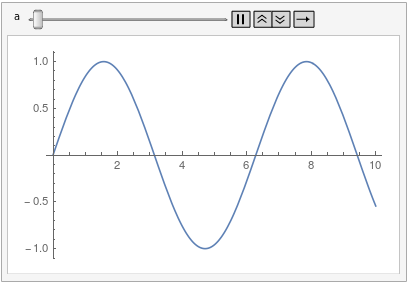
\includegraphics[scale=.5]{png/animaciones/sin/frame-0.png}
				\caption{Fija}
			\end{figure}
		}{
			\begin{figure}[H]
				\centering
				\animationswolfram{
					Animate[Plot[Sin[x + a], {x, 0, 10}], {a, 0, 5}]
				}{sin}{7cm}
				\caption{Animación con Wolfram}
			\end{figure}
		}
	\end{tcblisting}
	Finalmente con obtenemos que
	\begin{figure}[H]
		\centering
		\panimate{
			\begin{figure}[H]
				\centering
				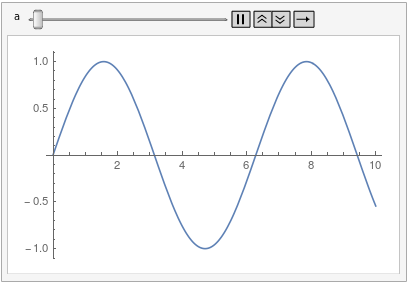
\includegraphics[scale=.5]{png/animaciones/sin/frame-0.png}
				\caption{Fija}
			\end{figure}
		}{
			\begin{figure}[H]
				\centering
				\animationswolfram{
					Animate[Plot[Sin[x + a], {x, 0, 10}], {a, 0, 5}]
				}{sin}{7cm}
				\caption{Animación con Wolfram}
			\end{figure}
		}
	\end{figure}
	\begin{boxbasic}
		Recuerde que la animación solo funciona en AdobeReader 9.0
	\end{boxbasic}
	}
%\nochapterimage